\section{Faza projektowania}
W tym rozdziale omówimy etap projektowania oraz ogólną architekturę aplikacji selfimprovement.ai. Przedstawimy moduły tworzące tę aplikację, ich wzajemne zależności oraz integrację z zewnętrznymi systemami. Architektura została opracowana zgodnie z modelem C4 (opisanym w kolejnym rozdziale 4.4), co pozwoli na klarowne przedstawienie struktury systemu oraz jego poszczególnych komponentów.

Aby ułatwić zrozumienie budowy naszego systemu stworzyliśmy również dodatkowy diagram wizualizujący architekturę systemu.

\begin{figure}[h]
    \centering
    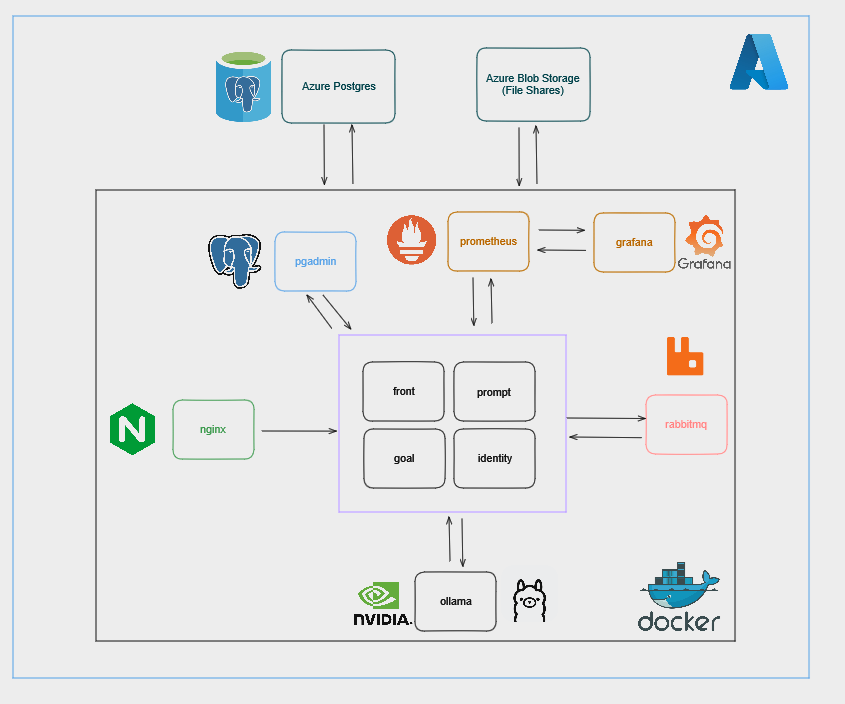
\includegraphics[width=0.95\textwidth]{Obrazy/architecture.png}
    \caption{Container Diagram}
    \label{fig:my_label}
\end{figure}

\subsection{Ogólny opis architektury}
Selfimprovement.ai to platforma internetowa, która umożliwia użytkownikom tworzenie spersonalizowanych planów na podstawie ich potrzeb oraz celów, takich jak plany treningowe, które pomagają użytkownikom zrealizować plan rozwoju w optymalnie zaplanowanym czasie. Aplikacja składa się z dwóch głównych części: front-endu i back-endu.

Front-end aplikacji selfimprovement.ai został napisany w React.js. Jest to popularne rozwiązanie do tworzenia aplikacji internetowych, które pozwala na budowanie szybkich, responsywnych i dynamicznie generowanych stron. W aplikacji selfimprovement.ai front-end odpowiada za prezentację danych oraz interakcję z użytkownikiem. Cała interakcja użytkownika z front-endem jest realizowana przy użyciu React.js, co umożliwia dynamiczne generowanie zawartości, takie jak strony do tworzenia celów, przeglądanie ich w kalendarzu czy analiza postępów. Dodatkowo, aplikacja wykorzystuje architekturę mikroserwisów, co pozwala na elastyczne i skalowalne zarządzanie różnymi funkcjonalnościami systemu.

\subsubsection{Mikroserwisy}

Mikroserwisy to architektoniczny wzorzec projektowy, który polega na budowaniu aplikacji jako zestawu małych, autonomicznych komponentów, które są niezależne od siebie pod względem wdrożenia i skalowania. Każdy mikroserwis odpowiada za realizację jednej konkretnej funkcji lub usługi, co pozwala na elastyczne zarządzanie aplikacją oraz umożliwia uniezależnienie się od monolitycznej architektury.

Pojawienie się architektury mikroserwisowej wynikało z konieczności przeciwdziałania wadom tradycyjnych, monolitycznych systemów aplikacyjnych. W starszych rozwiązaniach monolitycznych wszystkie funkcjonalności aplikacji są zintegrowane w jednym, złożonym kodzie, co prowadziło do problemów związanych z skalowaniem, utrzymaniem i rozwijaniem aplikacji.

Monolity na początku oferowały wygodę w zakresie rozwoju, wdrażania i utrzymania, że nawet najmniejsze zmiany w jednej części aplikacji wymagały ponownego wdrażania całego systemu. Dodatkowo, rozwój aplikacji wymagał współpracy między różnymi zespołami, co często prowadziło do konfliktów i opóźnień.

W odpowiedzi na te problemy, architektura mikroserwisowa została zaprojektowana jako alternatywa. W tym podejściu każda funkcja aplikacji jest implementowana jako oddzielny mikroserwis, komunikujący się ze sobą poprzez interfejsy programistyczne (API), co umożliwia niezależne wdrażanie, skalowanie i rozwijanie poszczególnych części aplikacji. Dzięki temu, nawet największe i najbardziej złożone aplikacje stają się bardziej elastyczne, skalowalne i łatwiejsze w utrzymaniu.

Architektura ta pozwala również na lepsze wykorzystanie zasobów sprzętowych poprzez niezależne skalowanie poszczególnych mikroserwisów w zależności od obciążenia, co prowadzi do lepszej wydajności i oszczędności kosztów operacyjnych. Dodatkowo, ułatwia ona wprowadzanie zmian i aktualizacji w aplikacji poprzez możliwość modyfikacji jednego komponentu bez wpływu na pozostałe.

Współczesne narzędzia, takie jak Docker czy Kubernetes, oraz platformy chmury obliczeniowej, umożliwiają efektywne zarządzanie i wdrażanie mikrousług, co stanowi kluczowy element nowoczesnych środowisk biznesowych.

\subsubsection{GitOps}
Podczas procesu wytwarzania oprogramowania zastosowaliśmy powszechne praktyki zgodne z kulturą i praktykami DevOps. Jedną z nich jest GitOps, czyli podejście do zarządzania infrastrukturą i aplikacjami, które traktuje kod źródłowy jako jedyną prawdę w procesie CI/CD. Wykorzystuje narzędzia takie jak Git do automatyzacji procesów wdrożeniowych, zapewniając przy tym spójność i przejrzystość konfiguracji dzięki wersjonowaniu i kodowi źródłowemu.

\subsubsection{Github}
Naszym repozytorium kodu została platforma Github, a narzędziem CI/CD "Github Actions", wybór rozwiązania wynikał głównie z dwóch czynników. Pierwszym czynnikiem było wcześniejsze nawyki oraz preferencje całego zespołu pracy z repozytorium kodu. Drugim integracja ze środowiskiem chmurowym Azure, ponieważ Github i jego wszystkie elementy należą do firmy Microsoft.

\subsubsection{Pipeline}
Pipeline w kontekście GitHub Actions to zautomatyzowany proces, który składa się z serii zadań (jobs), które są wykonywane po każdym zdarzeniu w repozytorium, takim jak push czy pull request. Każde zadanie może zawierać kroki (steps), które wykonują specyficzne akcje, takie jak kompilacja kodu, testy, aż do wdrożenia aplikacji, co pozwala na ciągłą integrację i dostarczanie oprogramowania.

\subsubsection{Monitoring}
Architektura mikroserwisów potrzebuje dobrego systemu monitoringu, ponieważ system w prównaniu do monolitu jest bardziej zdecentralizowany i potrzebuje dokładnej analizy różnych metryk takich jak: natężenie ruchu sieciowego, liczba wolnej pamięci RAM zużywanej przez dany serwis itp.

\subsubsection{Prometheus i Grafana}
Narzędzia takie jak Prometheus oraz Grafana są bardzo powszechne we współczesnych aplikacjach chmurowych. Prometheus to system monitoringu i alertowania, który zbiera i przechowuje metryki w czasie rzeczywistym w formie serii czasowych. Dane są zbierane za pomocą protokołu HTTP z różnych źródeł, takich jak serwery czy aplikacje, a następnie wyświetlane w programie Grafna, która umożliwia ich analizę i wizualizację za pomocą zapytań i grafów.

\subsubsection{RabbitMq}
Ważnym czynnikiem jest jak poszczególne komponenty aplikacji komunikują się ze sobą, ze względu na izolację zasobów muszą one się komunikować za pomocą wspólnego dla nich mechanizmu. RabbitMQ to popularny open-source'owy broker wiadomości, który umożliwia asynchroniczną komunikację między komponentami oprogramowania poprzez wymianę wiadomości. Umożliwia to tworzenie rozproszonych systemów, które są bardziej skalowalne i odporne na błędy, dzięki wykorzystaniu różnorodnych wzorców komunikacyjnych, takich jak publikowanie/subskrypcja czy kolejki.

\subsubsection{Zastosowane praktyki}
Nasze mikroserwisy opierają się o cztery autorskie kontenery, napisane w technologiach .Net oraz React, za pomocą odpowiednio napisanych pipelinów jesteśmy w stanie utworzyć proces który sprawdza konfigurację pliku "docker-compose", przeprowadzić walidację parametrów oraz dostarczyć niezbędne zmienne środowiskowe aby utworzyć własne obrazy Dockerowe. Przechowywane są one w Azure Container Registry (ACR), rozwiązanie zapewnia prywatne repozytorium kontenerów co jest prawidłową praktyką bezpieczeństwa we współczesnych systemach chmurowych.

\clearpage

\subsection{DevOps}

{\bf Synergia Pomiędzy Rozwojem a Operacjami:}

\noindent DevOps, skrócony od "Development" (rozwój) i "Operations" (operacje), to koncepcja i praktyka, która zakłada ścisłą współpracę między zespołami odpowiedzialnymi za rozwój oprogramowania (Dev) a tymi, które zajmują się operacjami IT (Ops). Celem DevOps jest skrócenie cyklu dostarczania oprogramowania, zwiększenie częstotliwości wdrożeń, poprawa stabilności systemów oraz usprawnienie komunikacji i współpracy między różnymi działami organizacji.
\\

{\noindent\bf Kluczowe Aspekty DevOps:} 
\begin{enumerate}
\item {\bf Automatyzacja}
   - Wykorzystanie narzędzi do automatyzacji procesów wytwarzania oprogramowania, testowania, wdrażania oraz monitorowania.
   - Automatyzacja pomaga zminimalizować błędy związane z interwencją ludzką i przyspiesza procesy.

\item {\bf Kontrola Wersji}
   - Korzystanie z systemów kontroli wersji, takich jak Git, w celu śledzenia zmian w kodzie źródłowym i ułatwienia współpracy pomiędzy członkami zespołu.

\item {\bf Konteneryzacja}
   - Wykorzystanie technologii konteneryzacji, na przykład Docker, umożliwiającej pakowanie oprogramowania w izolowane jednostki, co ułatwia przenośność i wdrażanie aplikacji.

\item {\bf Infrastruktura Jako Kod (IaaC)}
   - Traktowanie infrastruktury jak kodu programistycznego, co umożliwia jej zarządzanie, wdrażanie i skalowanie przy użyciu praktyk znanym z programowania.

\item {\bf Kultura i Współpraca}
   - Zmiana kultury organizacyjnej, promowanie współpracy i komunikacji pomiędzy zespołami Dev i Ops.
   - Eliminacja barier i podziałów, tworząc zintegrowane zespoły mające wspólny cel.

\item {\bf Monitorowanie i Analiza}
   - Utrzymywanie ciągłego monitorowania działania systemu, zbieranie danych, analiza i reakcja na ewentualne problemy.
\end{enumerate}

\clearpage

\noindent{\bf Korzyści DevOps:}

\begin{enumerate}
\item {\bf Skrócenie Cyklu Dostarczania}
   - Dzięki automatyzacji i zintegrowanym procesom, czas potrzebny na dostarczenie nowej funkcjonalności lub poprawki zostaje znacznie zredukowany.

\item {\bf Zwiększenie Stabilności}
   - Stałe monitorowanie i automatyczne testowanie pomagają zminimalizować ryzyko błędów oraz poprawiają stabilność i niezawodność systemów.

\item {\bf Elastyczność i Skalowalność}
   - Konteneryzacja i elastyczne zarządzanie infrastrukturą umożliwiają łatwe skalowanie zasobów w zależności od potrzeb.

\item {\bf Efektywność Kosztowa}
   - Automatyzacja procesów i bardziej efektywne zarządzanie zasobami przekładają się na oszczędności czasu i środków.
\end{enumerate}

W skrócie, DevOps stanowi holistyczne podejście do wytwarzania oprogramowania, łączące aspekty kulturowe, procesowe i technologiczne w celu stworzenia efektywnego i responsywnego środowiska IT.

\subsubsection{Opis technologii}

\begin{enumerate}

\item {\bf Docker} - Jest narzędziem do zarządzania kontenerami, które pozwala na pakowanie aplikacji wraz z ich zależnościami w lekkie, przenośne, samowystarczalne kontenery, które mogą być łatwo przemieszczane między różnymi środowiskami. Umożliwia to szybkie wdrażanie oraz skalowanie aplikacji w różnorodnych środowiskach.

\item {\bf Kubernetes} - To otwartoźródłowy system do automatyzacji wdrażania, skalowania oraz zarządzania aplikacjami kontenerowymi. Kubernetes umożliwia łatwą orkiestrację kontenerów, zarządzanie cyklem życia aplikacji oraz zapewnia wysoką dostępność i skalowalność usług.

\item {\bf Kind} - Jest narzędziem służącym do uruchamiania lokalnych klastrów Kubernetesowych za pomocą Dockera. Idealnie nadaje się do testowania w izolowanym środowisku na pojedynczym komputerze, co jest przydatne w testowaniu aplikacji przed etapem zaimplementowania jej w architekturze chmurowej.

\item {\bf Azurite} - Jest lekkim, otwartoźródłowym emulatorem usług magazynowych Azure, który pozwala na lokalne uruchamianie i testowanie aplikacji korzystających z usług Azure Storage bez konieczności dostępu do chmury Azure, co jest przydatne w fazie rozwoju i testów.

\item {\bf Powershell} - To zaawansowany język skryptowy i środowisko powłoki zaprojektowane przez Microsoft dla systemów Windows, które umożliwia zautomatyzowanie zarządzania systemem oraz aplikacjami. Powershell jest wyposażony w potężne narzędzia do manipulacji obiektami i integracji z innymi technologiami.

\item {\bf Bash} - Jest jednym z najpopularniejszych języków skryptowych dla powłoki systemów typu Unix, który umożliwia skuteczne zarządzanie systemem oraz automatyzację zadań za pomocą prostych skryptów. Bash jest ceniony za swoją prostotę i mocne wsparcie w środowiskach Linux i macOS oraz w kontenerach Dockerowych.

\item {\bf Terraform} - Jest narzędziem do zarządzania infrastrukturą jako kodem, które pozwala na definiowanie i wdrażanie infrastruktury w różnych dostawcach usług chmurowych za pomocą prostego języka konfiguracyjnego. Terraform jest wykorzystywany do budowy, zmian i wersjonowania infrastruktury bezpiecznie i efektywnie.

\item {\bf Azure KeyVault} - Jest to usługa zarządzania kluczami i sekretami, która pozwala na bezpieczne przechowywanie danych poufnych, takich jak klucze szyfrowania, certyfikaty oraz hasła. Dzięki Azure KeyVault, aplikacje mogą bezpiecznie uzyskiwać dostęp do potrzebnych haseł oraz kluczy bez konieczności ich jawnej ekspozycji w kodzie, co znacznie zwiększa bezpieczeństwo i zarządzanie danymi poufnymi.

\end{enumerate}

\subsubsection{CI/CD}
{\bf Ciągła Integracja i Ciągłe Dostarczanie/Dostosowywanie:}

\noindent CI/CD to skrót od dwóch kluczowych praktyk w inżynierii oprogramowania: Ciągłej Integracji (Continuous Integration) i Ciągłego Dostarczania/Dostosowywania (Continuous Delivery/Continuous Deployment). Te praktyki są ważnymi elementami podejścia DevOps, mającym na celu skrócenie cyklu dostarczania oprogramowania i poprawę jakości wytwarzanego kodu.
\\

\noindent{\bf Ciągła Integracja (CI):}

\noindent Ciągła Integracja odnosi się do praktyki regularnego i automatycznego łączenia zmian wprowadzanych przez różnych członków zespołu programistycznego do wspólnego repozytorium kodu. Głównym celem CI jest wczesne wykrywanie i rozwiązywanie konfliktów oraz zapewnienie, że kod jest zawsze w spójnym i testowalnym stanie. Kluczowymi elementami CI są:

\begin{enumerate}
\item {\bf Automatyczne Budowanie (Build)}
- Automatyzacja procesu kompilacji i budowy aplikacji po wprowadzeniu nowych zmian.

\item {\bf Automatyczne Testowanie (Test)}
   - Wykonywanie automatycznych testów jednostkowych, integracyjnych oraz innych, aby zweryfikować, czy wprowadzone zmiany nie wprowadzają błędów.

\item {\bf Ciągła Weryfikacja Kodu (Code Quality)}
   - Analiza jakości kodu poprzez narzędzia sprawdzające zgodność z ustalonymi standardami.
\end{enumerate}

\noindent{\bf Ciągłe Dostarczanie (CD) i Ciągłe Dostosowywanie (CD):}

\noindent Ciągłe Dostarczanie i Ciągłe Dostosowywanie to dwa powiązane, ale różniące się podejścia do dostarczania oprogramowania do produkcji.

\begin{enumerate}
\item {\bf Ciągłe Dostarczanie (Continuous Delivery - CD)}
   - Proces, w którym każda zmiana w kodzie, która przejdzie przez etap CI, jest automatycznie gotowa do dostarczenia do produkcji.
   - Ręczne potwierdzenie może być wymagane przed finalnym wdrożeniem, ale sama procedura dostarczania jest zautomatyzowana.

\item {\bf Ciągłe Dostosowywanie (Continuous Deployment - CD)}
   - Bardziej radykalne podejście, w którym każda zmiana, która przejdzie przez etap CI, jest automatycznie wdrażana w środowisku produkcyjnym bez ręcznej interwencji.
\end{enumerate}

\noindent{\bf Korzyści CI/CD:}

\begin{enumerate}
\item {\bf Skrócenie Cyklu Dostarczania}
   - Automatyzacja procesów przyspiesza cykl dostarczania oprogramowania.

\item {\bf Poprawa Jakości}
   - Systematyczne testowanie i weryfikacja kodu przyczyniają się do poprawy jakości oprogramowania.

\item {\bf Elastyczność i Odporność na Błędy}
   - Automatyczne wdrażanie ułatwia wprowadzanie zmian oraz umożliwia szybką reakcję na ewentualne problemy.

\item {\bf Zwiększenie Efektywności}
   - Redukcja czasu i nakładu pracy związanych z ręcznymi procesami wytwarzania i wdrażania oprogramowania.
\end{enumerate}

W sumie, CI/CD to kluczowy element podejścia DevOps, przyczyniający się do bardziej efektywnego, responsywnego i jakościowego dostarczania oprogramowania.
\subsubsection{Kubernetes}

{\bf Orkiestracja Kontenerów dla Skalowalnych i Zdecentralizowanych Aplikacji}

\noindent Kubernetes, często nazywany "K8s" (gdzie "8s" oznacza osiem liter 'ubernete'), to popularna platforma do automatyzacji, zarządzania i orkiestracji kontenerów. Kontenery są lekkimi, przenośnymi jednostkami uruchomieniowymi, a Kubernetes ułatwia zarządzanie ich cyklem życia, skalowaniem i dystrybucją w rozproszonych środowiskach.
\\

{\bf Podstawowe Koncepcje Kubernetes:}

\begin{enumerate}
\item {\bf Kontener}
   - Izolowana jednostka, która zawiera aplikację i jej zależności, co umożliwia przenośność i jednolitość środowiska wykonawczego.

\item {\bf Pod}
   - Najmniejsza jednostka w środowisku Kubernetes, składająca się z jednego lub wielu kontenerów, które współdzielą zasoby i przestrzeń sieciową.

\item {\bf Węzeł (Node)}
   - Fizyczna lub wirtualna maszyna, na której uruchamiane są kontenery. Węzły stanowią infrastrukturę, na której działa klastr Kubernetes.

\item {\bf Klastr}
   - Zbiór węzłów, które współpracują w celu uruchamiania i zarządzania kontenerami.

\item {\bf Kontroler}
   - Element zarządzający cyklem życia podów, np. Deployment Controller, ReplicaSet Controller, czy DaemonSet Controller.

\item {\bf Usługa:}
   - Abstrakcja, która umożliwia dostęp do zestawu podów, oferując trwały adres IP i nazwę hosta.

\item {\bf Przestrzeń Nazw (Namespace)}
   - Sposób na grupowanie i izolację zasobów w klastrze. Umożliwia tworzenie logicznych segmentów w klastrze.
\end{enumerate}

{\bf Funkcje i Zastosowania Kubernetes:}

\begin{enumerate}
\item {\bf Orkiestracja}
   - Automatyczne zarządzanie cyklem życia kontenerów, w tym ich uruchamianiem, zatrzymywaniem i skalowaniem.

\item {\bf Skalowalność}
   - Możliwość dynamicznego dostosowywania liczby instancji kontenerów w zależności od obciążenia aplikacji.

\item {\bf Równoważenie Obciążenia}
   - Rozdział ruchu sieciowego między różnymi instancjami kontenerów, aby zoptymalizować dostępność i wydajność.

\item {\bf Zarządzanie Konfiguracją}
   - Automatyczne dostosowywanie konfiguracji aplikacji bez potrzeby zatrzymywania i uruchamiania kontenerów.

\item {\bf Dystrybucja i Wersjonowanie}
   - Kontrola wersji aplikacji, ułatwiająca wprowadzanie zmian i aktualizacji bezprzerwowego dostarczania.

\item {\bf Bezpieczeństwo}
   - Mechanizmy kontroli dostępu, zarządzania tożsamością oraz izolacji podów dla zwiększenia bezpieczeństwa.
\end{enumerate}

{\bf Korzyści Korzystania z Kubernetes:}

\begin{enumerate}
\item {\bf Elastyczność i Skalowalność}
   - Łatwe skalowanie i zarządzanie zasobami, co umożliwia dostosowanie klastra do zmieniających się potrzeb.

\item {\bf Trwałość i Niezawodność}
   - Automatyczna naprawa i przenoszenie podów w przypadku awarii, zapewniając ciągłość działania aplikacji.

\item {\bf Jednolite Środowisko}
   - Zapewnienie jednolitego środowiska uruchomieniowego dla kontenerów niezależnie od lokalizacji czy infrastruktury.

\item {\bf Automatyzacja i Współpraca}
   - Ułatwienie automatyzacji procesów wytwarzania oprogramowania oraz współpracy między zespołami Dev i Ops.
\end{enumerate}

Kubernetes stał się fundamentalnym narzędziem w świecie kontenerów, pomagając organizacjom osiągnąć elastyczność, niezawodność i skalowalność ich aplikacji w środowiskach chmurowych i lokalnych.
\subsubsection{Monitorowanie aplikacji}

\noindent{\bf Kluczowy Element Zarządzania i Utrzymania Wysokiej Jakości Systemów}

\noindent Monitorowanie aplikacji to proces zbierania, analizy i interpretacji danych dotyczących działania aplikacji w celu zapewnienia wydajności, niezawodności oraz efektywności operacyjnej. Skuteczne monitorowanie jest kluczowym elementem w zarządzaniu systemami informatycznymi, umożliwiając szybkie wykrywanie, diagnozowanie i rozwiązywanie potencjalnych problemów.
\\

\noindent{\bf Elementy Składowe Monitorowania Aplikacji:}

\begin{enumerate}
\item {\bf Logi Aplikacyjne}
   - Rejestracja zdarzeń i informacji z działania aplikacji w celu analizy błędów, śledzenia działań użytkowników oraz audytu.

\item {\bf Metryki Aplikacyjne}
   - Liczby, statystyki i wskaźniki mierzące wydajność i zachowanie aplikacji, takie jak czas odpowiedzi, zużycie zasobów czy ilość błędów.

\item {\bf Śledzenie Zdarzeń (Tracing)}
   - Monitorowanie ścieżki wykonania żądania poprzez aplikację, co ułatwia identyfikację i analizę opóźnień czy błędów.

\item {\bf Infrastruktura i Zasoby}
   - Monitorowanie stanu fizycznych i wirtualnych zasobów, takich jak CPU, pamięć RAM, dyski, sieć, aby ocenić wydajność i dostępność infrastruktury.

\item {\bf Alarmy i Powiadomienia}
   - Ustawianie alertów na podstawie ustalonych progów, które informują o potencjalnych problemach, umożliwiając szybką reakcję.
\end{enumerate}

\noindent{\bf Cele Monitorowania Aplikacji:}

\begin{enumerate}
\item {\bf Wczesne Wykrywanie Problemów}
   - Monitorowanie pozwala na szybkie identyfikowanie i diagnozowanie potencjalnych problemów, zanim wpłyną negatywnie na użytkowników.
   
\item {\bf Optymalizacja Wydajności}
   - Analiza metryk i logów umożliwia optymalizację wydajności aplikacji poprzez identyfikację obszarów wymagających ulepszeń.

\item {\bf Zarządzanie Zasobami}
   - Monitorowanie infrastruktury pozwala na efektywne zarządzanie zasobami, skalowanie w odpowiedzi na obciążenie oraz unikanie zbędnych kosztów.

\item {\bf Zapewnienie Dostępności}
   - Śledzenie dostępności aplikacji i jej komponentów, co pozwala na szybkie reagowanie na ewentualne awarie i minimalizowanie czasu niedostępności.

\item {\bf Planowanie Pojemności}
   - Analiza trendów zużycia zasobów pozwala na prognozowanie potrzeb pojemnościowych i planowanie przyszłych rozszerzeń.
\end{enumerate}

\noindent{\bf Popularne Narzędzia do Monitorowania Aplikacji:}

\begin{enumerate}
\item {\bf Prometheus}
   - Otwarte źródło, przeznaczone do monitorowania metryk i alarmów.

\item {\bf Grafana}
   - Narzędzie do wizualizacji danych monitorowania, integrujące się z różnymi źródłami danych.
\end{enumerate}

\noindent{\bf Wnioski:}

\noindent Monitorowanie aplikacji to nieodłączny element utrzymania nowoczesnych systemów informatycznych. Skuteczne monitorowanie pozwala na szybką reakcję na problemy, optymalizację wydajności oraz efektywne zarządzanie zasobami, przyczyniając się do zapewnienia niezawodności i satysfakcji użytkowników.
\clearpage

\subsection{Baza danych}
PostgreSQL, często po prostu "Postgres", to system zarządzania obiektowo-relacyjnymi bazami danych (ORDBMS) z naciskiem na rozszerzalność i zgodność ze standardami. Jako serwer bazy danych, jego podstawową funkcją jest przechowywanie danych, bezpieczne i wspierające najlepsze praktyki, oraz późniejsze ich pobieranie, zgodnie z wymaganiami innych aplikacji, zarówno tych na tym samym komputerze, jak i tych uruchomionych na innym komputerze w sieci (w tym w Internecie). Może obsługiwać obciążenia od małych aplikacji na jednym komputerze do dużych aplikacji internetowych z wieloma jednoczesnymi użytkownikami. Najnowsze wersje zapewniają również replikację samej bazy danych w celu zapewnienia bezpieczeństwa i skalowalności.

\subsubsection{Nginx}
Nginx (wymawiane "engine-x") to potężny serwer WWW, serwer odwrotne-proxy i równoważnik obciążenia. Pierwotnie stworzony przez Igora Sysoeva w 2004 roku, aby rozwiązać problem C10k (obsługi ponad 10 000 równoczesnych połączeń), Nginx zdobył powszechne uznanie ze względu na swoją wydajność, skalowalność i wszechstronność.
\\

\noindent{\bf Główne cechy Nginx obejmują:}

\begin{enumerate}
\item {\bf Wysoką wydajność: }
Nginx jest znany ze swojej efektywności w obsłudze równoczesnych połączeń i żądań, co czyni go odpowiednim do obsługi witryn internetowych i aplikacji o dużej liczbie odwiedzin.

\item {\bf Proxy odwrotny:}
Nginx może działać jako proxy odwrotne, siedząc przed serwerami WWW, aby obsłużyć przychodzące żądania klientów. Może rozprowadzać te żądania do wielu serwerów backendowych na podstawie różnych kryteriów, takich jak algorytmy równoważenia obciążenia, stan serwera lub lokalizacja geograficzna.

\item {\bf Równoważenie obciążenia: }
Nginx obejmuje możliwości równoważenia obciążenia, pozwalając na rozprowadzenie przychodzącego ruchu na wiele serwerów w celu poprawy niezawodności, skalowalności i wydajności.

\item {\bf Serwer HTTP:} 
Nginx efektywnie obsługuje treści statyczne i może być również skonfigurowany do obsługi treści dynamicznych za pomocą różnych modułów, w tym FastCGI, SCGI i uwsgi.

\item {\bf Zakończenie SSL/TLS:}
Nginx może obsługiwać zakończenie SSL/TLS, rozładowując proces szyfrowania i deszyfrowania z serwerów backendowych, poprawiając tym samym wydajność.

\item {\bf Pamięć podręczna proxy odwróconego:}
Nginx może buforować treści statyczne i dynamiczne w pamięci lub na dysku, zmniejszając obciążenie serwerów backendowych i poprawiając czasy odpowiedzi dla klientów.

\item {\bf Obsługa HTTP/2 i HTTP/3:}
Nginx obsługuje nowoczesne protokoły HTTP, w tym HTTP/2 i HTTP/3, które oferują lepszą wydajność i bezpieczeństwo w porównaniu do starszych wersji.

\item {\bf Bezpieczeństwo:}
Nginx zawiera funkcje zapobiegające powszechnym zagrożeniom dla bezpieczeństwa sieci, takim jak ataki DDoS, wstrzykiwanie SQL i skrypty między witrynami (XSS).
\end{enumerate}

Nginx jest powszechnie używany przez programistów internetowych, administratorów systemów i specjalistów DevOps do budowy skalowalnych, wysoko wydajnych aplikacji internetowych i usług. Jest znany z lekkiej architektury, niskiego zużycia zasobów i łatwości konfiguracji, co czyni go popularnym wyborem dla szerokiego zakresu zastosowań, od małych witryn do rozległych rozproszonych systemów.
\clearpage

\subsection{Model C4}
Model C4 to narzędzie służące do opisywania i komunikowania architektury aplikacji. W niniejszym rozdziale omówimy jego zastosowanie w kontekście naszej aplikacji selfimprovement.ai. Przedstawimy składniki naszej aplikacji, ich wzajemne powiązania oraz integracje z zewnętrznymi systemami.\\

Model C4 składa się z czterech poziomów abstrakcji: Context, Container, Component oraz Code. Poziom Context prezentuje kontekst, w jakim działa aplikacja oraz jej relacje z otoczeniem. Poziom Container obejmuje kontenery, w których znajdują się poszczególne komponenty aplikacji. Poziom Component opisuje komponenty aplikacji, ich interfejsy oraz wzajemne zależności. Poziom Code prezentuje implementację kodu poszczególnych komponentów. W dalszej części rozdziału przedstawimy każdy z tych poziomów abstrakcji na przykładzie naszej aplikacji.
\\

\noindent{\bf Diagram Context} - to graficzna reprezentacja całego systemu wraz z jego otoczeniem i kontekstem, w jakim działa aplikacja.

\begin{figure}[h]
    \centering
    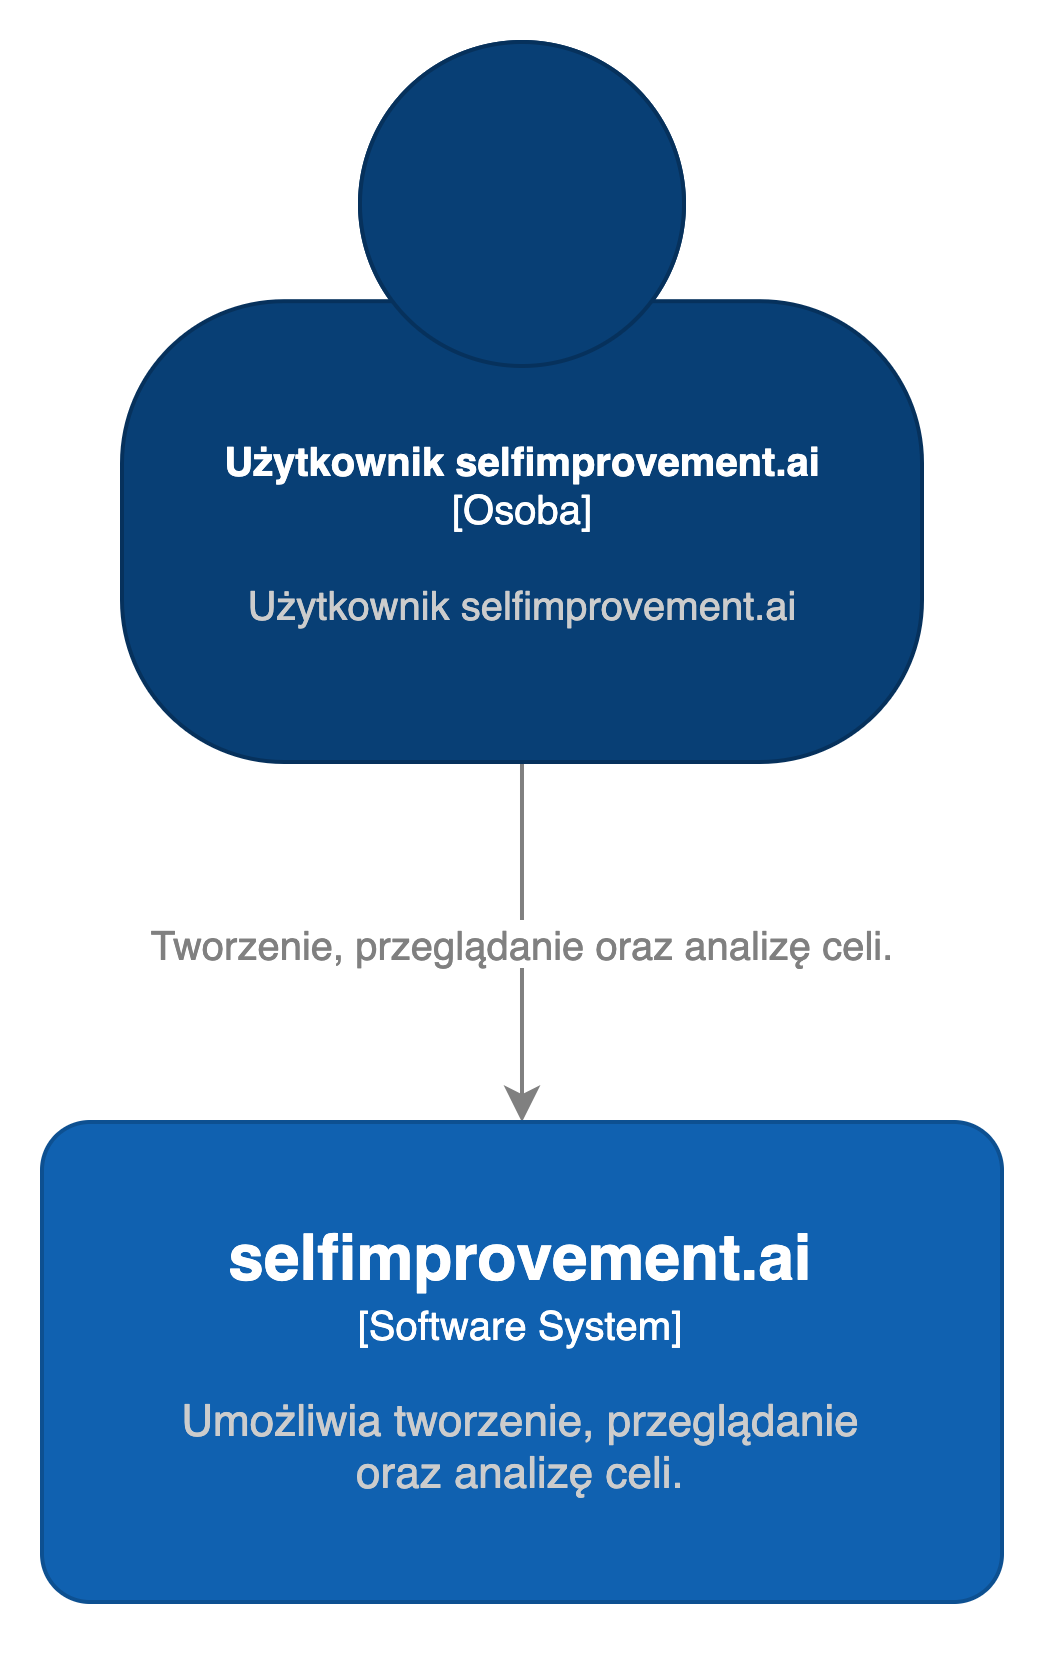
\includegraphics[width=0.4\textwidth]{Obrazy/c4_model/context_diagram.png}
    \caption{Context Diagram}
    \label{fig:my_label}
\end{figure}
\clearpage

\noindent{\bf Diagram Container} - przedstawia kontenery zawierające komponenty aplikacji oraz opisuje ich rolę i wzajemne zależności.

\begin{figure}[h]
    \centering
    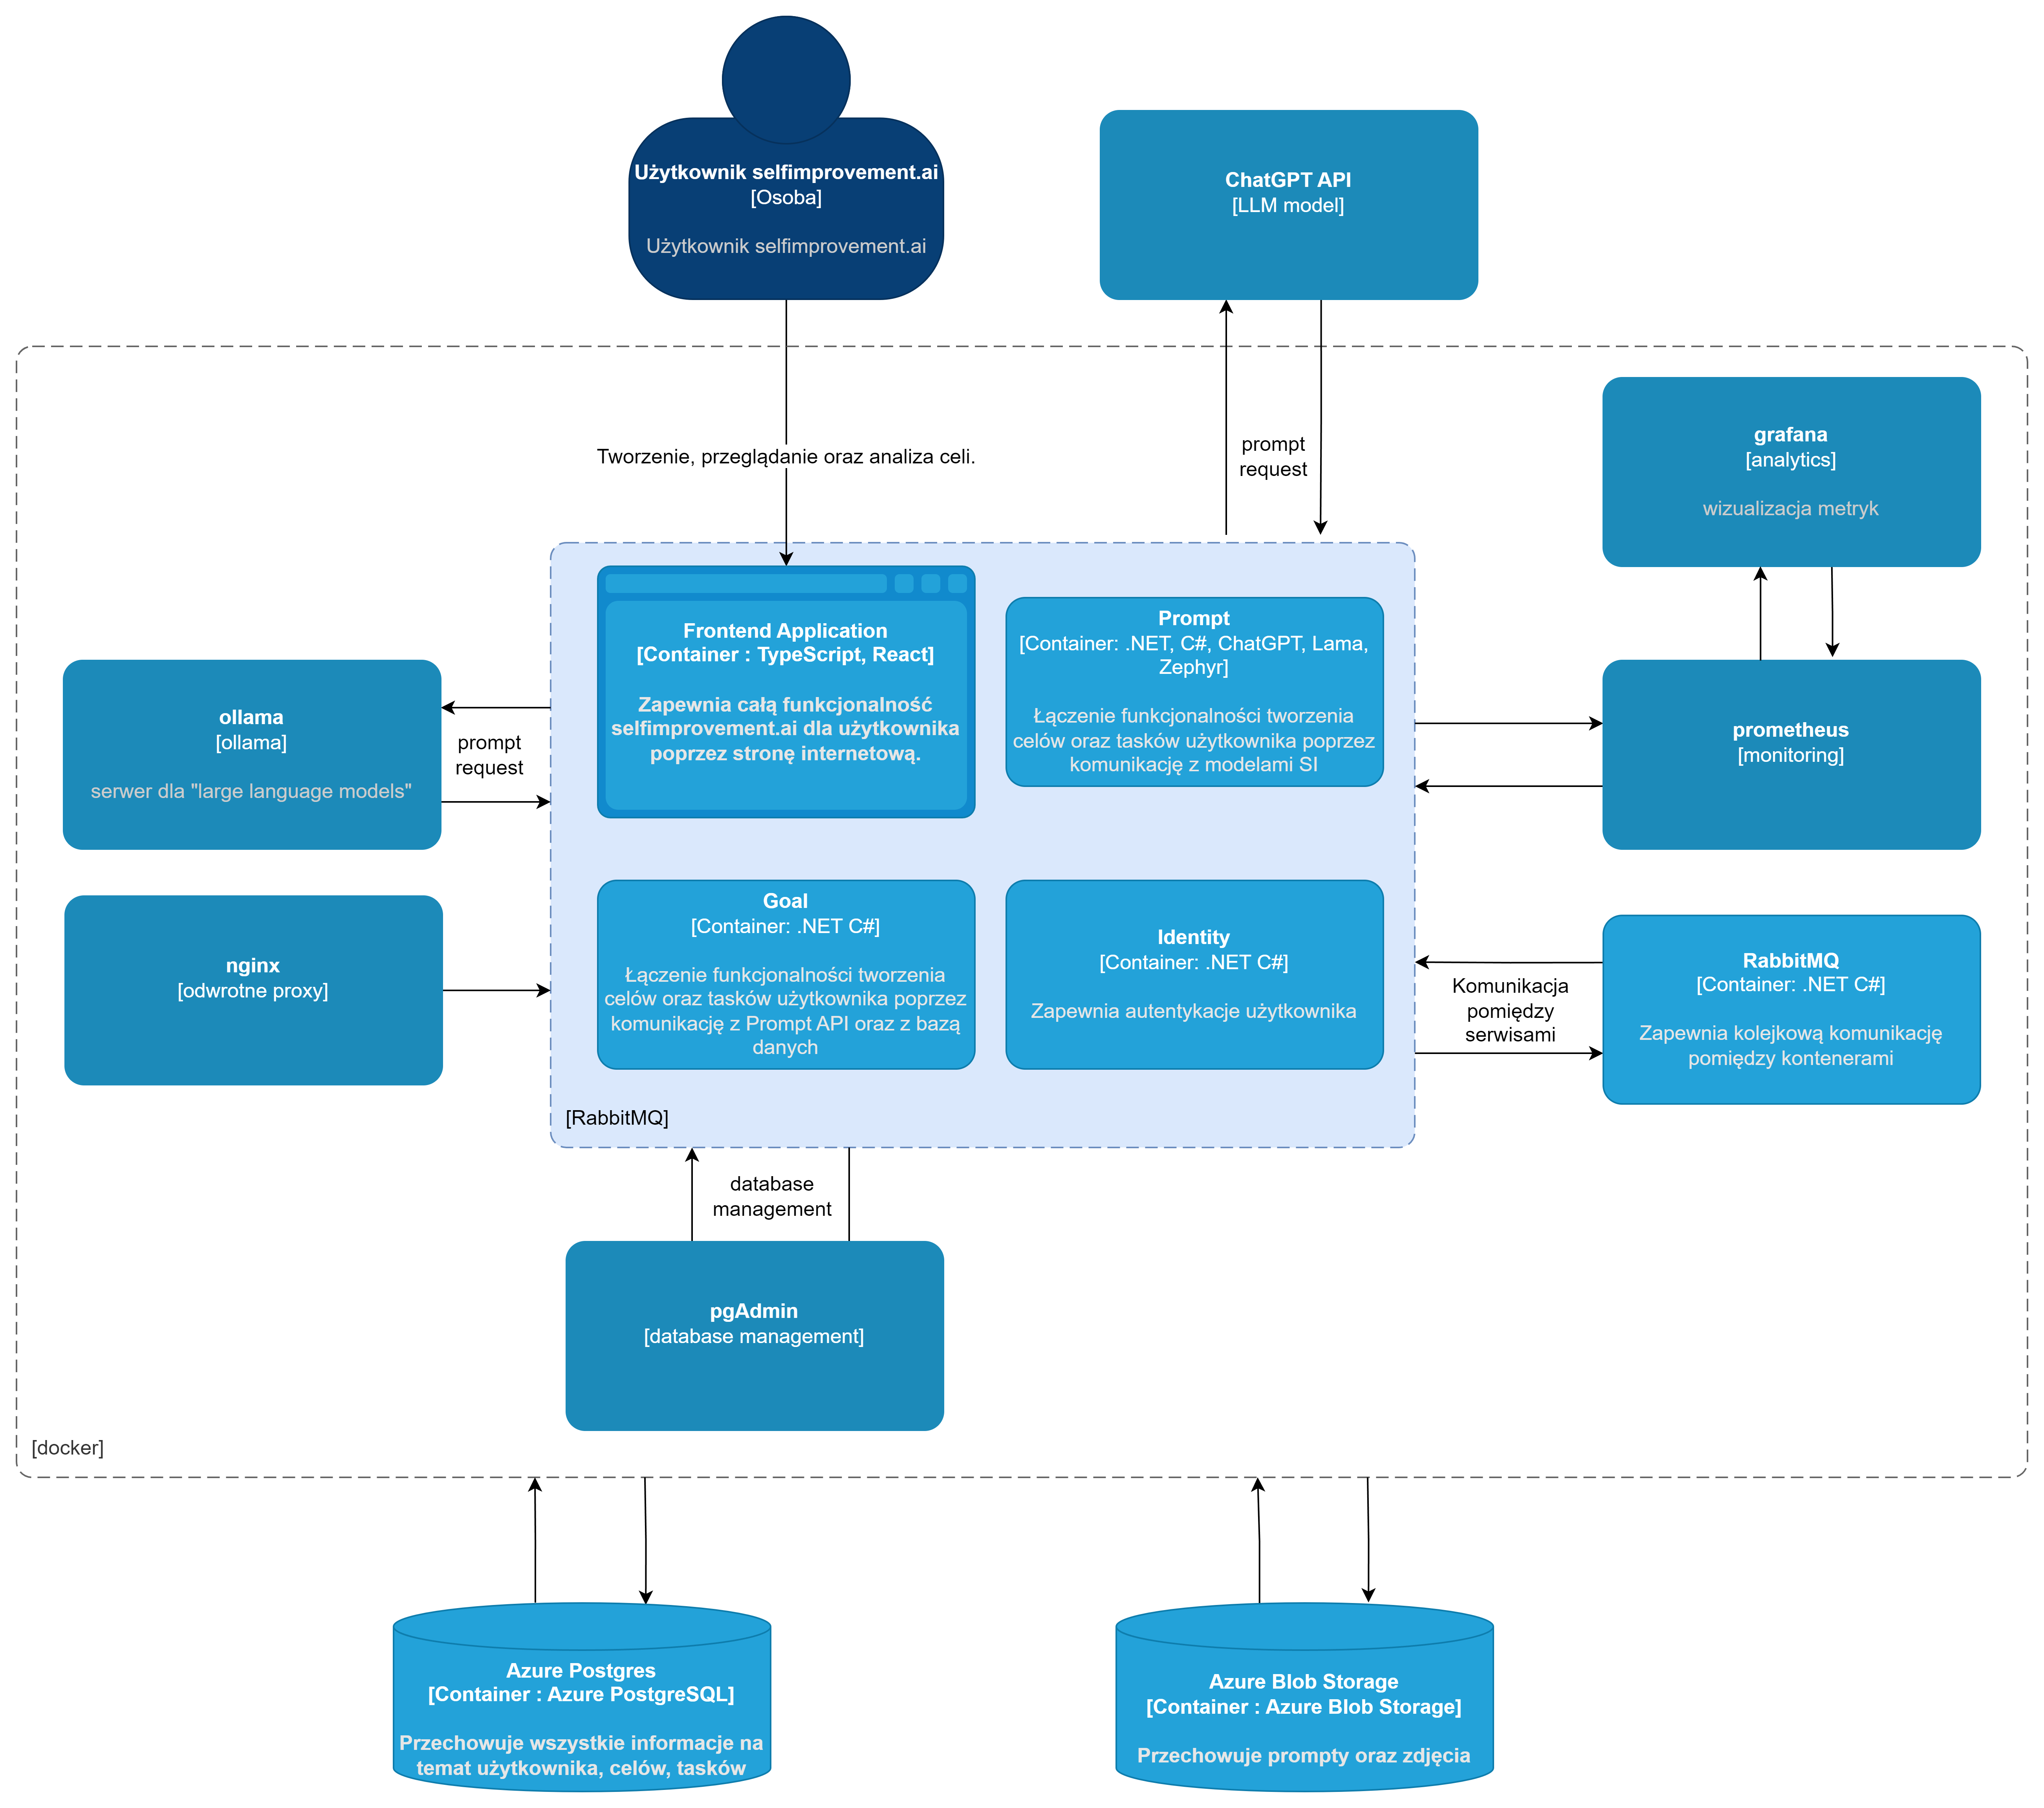
\includegraphics[width=0.95\textwidth]{Obrazy/c4_model/container_diagram.png}
    \caption{Container Diagram}
    \label{fig:my_label}
\end{figure}
\clearpage

\noindent{\bf Diagram Component} - prezentuje poszczególne komponenty aplikacji, ich interfejsy oraz wzajemne powiązania.

\begin{figure}[h]
    \centering
    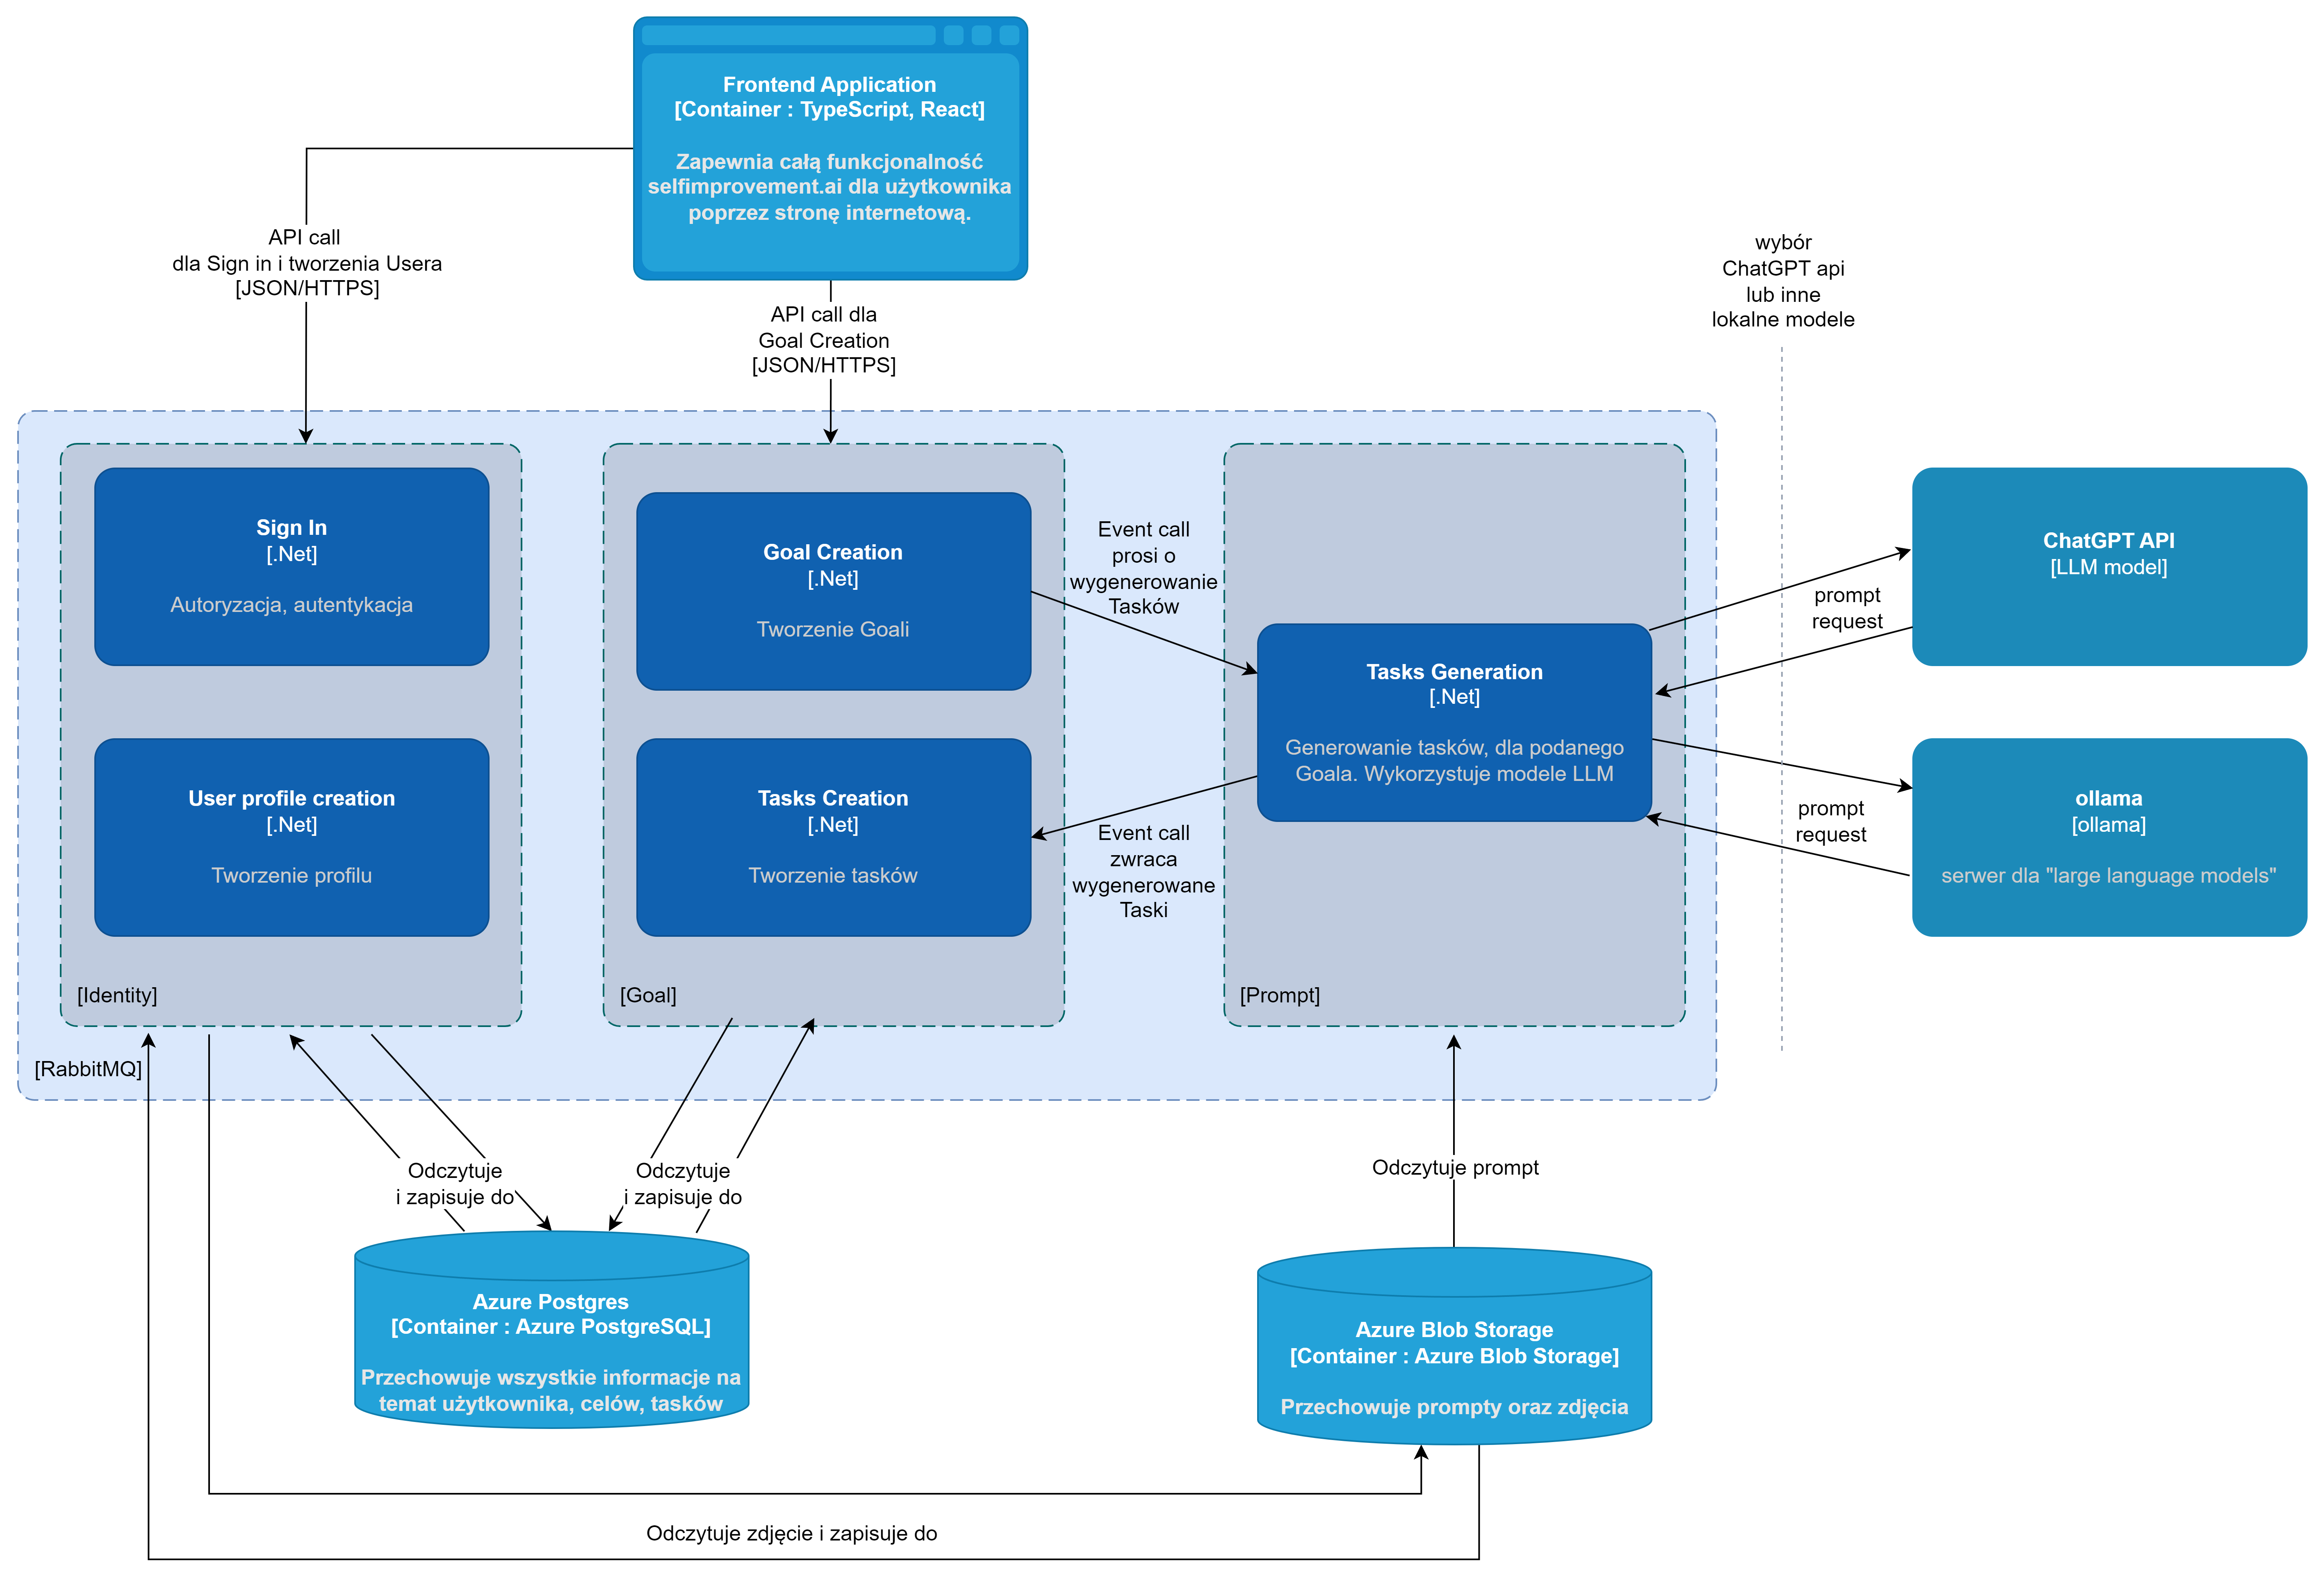
\includegraphics[width=1.1\textwidth]{Obrazy/c4_model/component_diagram.png}
    \caption{Component Diagram}
    \label{fig:my_label}
\end{figure}

Model C4 okazał się niezwykle przydatnym narzędziem do opisu architektury naszej aplikacji selfimprovement.ai. Przeanalizowaliśmy składniki aplikacji oraz ich zależności na poziomach Context, Container i Component, co pozwoliło nam lepiej zrozumieć strukturę systemu. Diagramy Context, Container i Component były kluczowe w ułatwieniu komunikacji w zespole oraz planowaniu architektury i implementacji. Wnioski z zastosowania Modelu C4 przyczyniły się do bardziej efektywnego projektowania, rozwijania i utrzymywania aplikacji poprzez lepsze zarządzanie złożonością systemu oraz usprawnienie komunikacji w całym zespole programistycznym.
\clearpage

\subsection{Aplikacja front-endowa}
Frontend w kontekście aplikacji webowych odgrywa kluczową rolę, stanowiąc interfejs użytkownika, który jest pierwszym punktem kontaktu z aplikacją. Jest to warstwa, którą użytkownicy widzą i z nią interakcjonują, obejmująca prezentację danych oraz funkcjonalności, które umożliwiają użytkownikom wygodne korzystanie z aplikacji. Frontend musi być zarówno estetyczny, jak i intuicyjny, aby zapewnić pozytywne wrażenia użytkownika oraz skuteczną realizację celów aplikacji.

Tworzenie frontendu to proces kompleksowy, który wymaga zrozumienia potrzeb użytkowników, projektowania interfejsu użytkownika oraz implementacji odpowiednich funkcjonalności. Współczesne technologie frontendowe, takie jak TypeScript, React, Material-UI (MUI) i SCSS, zapewniają programistom narzędzia i biblioteki umożliwiające efektywne tworzenie nowoczesnych i interaktywnych interfejsów użytkownika.

W niniejszym rozdziale przyjrzymy się bliżej procesowi tworzenia frontendu w aplikacji webowej, skupiając się na roli i znaczeniu użytych przez nas technologii. Przeanalizujemy, jak te narzędzia mogą być wykorzystane w praktyce do projektowania i implementacji atrakcyjnych oraz funkcjonalnych interfejsów użytkownika. Poprzez zrozumienie procesu tworzenia frontendu oraz korzyści płynących z wykorzystania zaawansowanych technologii, będziemy mogli lepiej zrozumieć rolę frontendu w kontekście aplikacji webowych oraz skuteczniej realizować cele projektowe.

\subsubsection{Opis bibliotek i frameworków}

\begin{enumerate}

    \item {\bf JavaScript} - jest dynamicznym, interpretowanym językiem programowania, który jest powszechnie używany do tworzenia interaktywnych aplikacji internetowych. Jest to język skryptowy, który działa po stronie klienta (w przeglądarce internetowej), co umożliwia tworzenie interaktywnych elementów, animacji oraz obsługę zdarzeń. JavaScript jest niezbędny do implementacji funkcjonalności frontendowych, takich jak manipulacja DOM (Document Object Model), obsługa formularzy, walidacja danych oraz komunikacja z serwerem za pomocą asynchronicznych żądań AJAX.
    
    \item {\bf TypeScript} - to nadzbiór języka JavaScript, który dodaje statyczną typizację, co znacząco zwiększa bezpieczeństwo oraz czytelność kodu. Dzięki TypeScriptowi programiści mogą definiować typy danych oraz interfejsy, co ułatwia wykrywanie błędów podczas kompilacji. Ponadto, TypeScript oferuje bogate narzędzia do refaktoryzacji kodu oraz zapewnia lepsze wsparcie dla środowisk programistycznych, co przekłada się na wyższą produktywność i jakość aplikacji. Jego elastyczność i skalowalność czynią go popularnym wyborem przy tworzeniu aplikacji webowych o większej złożoności.
    
    \item {\bf React.js} - to biblioteka JavaScript stworzona przez Facebook (Meta), służąca do budowy interfejsów użytkownika. Dzięki Reactowi możliwe jest tworzenie aplikacji, które dynamicznie reagują na zmiany danych w czasie rzeczywistym, co przekłada się na szybkość i efektywność działania aplikacji. Centralnym konceptem w React jest tworzenie komponentów, które stanowią niezależne i niezawodne elementy interfejsu użytkownika.
    
    \item {\bf MUI} - to popularna biblioteka komponentów interfejsu użytkownika dla aplikacji internetowych, oparta na zasadach Material Design. Zawiera zestaw gotowych i stylowych komponentów, takich jak przyciski, formularze, paski nawigacyjne i wiele innych, które można łatwo integrować w projekcie. MUI zapewnia nie tylko estetyczny wygląd, ale także zapewnia spójność wizualną i użytkową między różnymi częściami aplikacji. Ponadto, Material-UI oferuje elastyczność i konfigurowalność komponentów, co pozwala programistom dostosować interfejs do indywidualnych potrzeb projektu. Dzięki dużej popularności i aktywnej społeczności wsparcia, Material-UI stał się jednym z najczęściej wybieranych narzędzi przy tworzeniu nowoczesnych i atrakcyjnych interfejsów użytkownika w aplikacjach webowych.
    
    \item {\bf SCSS} - jest preprocesorem CSS, który wprowadza dodatkowe funkcje i możliwości do standardowego języka CSS. Dzięki SCSS można pisać bardziej czytelny i łatwiejszy do zarządzania kod CSS poprzez zastosowanie zmiennych, zagnieżdżania, mixinów oraz funkcji. Zmienne pozwalają na definiowanie wartości, które mogą być wielokrotnie używane w kodzie, co ułatwia utrzymanie spójności wizualnej i szybką zmianę wyglądu całej aplikacji. Zagnieżdżanie umożliwia definiowanie stylów dla zagnieżdżonych elementów HTML, co sprawia, że kod jest bardziej zorganizowany i czytelny. Mixiny pozwalają na zdefiniowanie zestawów stylów, które mogą być używane wielokrotnie, co eliminuje powtarzalność kodu i ułatwia jego utrzymanie. Dodatkowo, SCSS oferuje możliwość korzystania z zaawansowanych funkcji matematycznych oraz logiki, co czyni go bardziej elastycznym i potężnym narzędziem przy tworzeniu zaawansowanych stylów CSS. Dzięki swojej popularności i wsparciu przez wiele narzędzi deweloperskich, SCSS stał się standardem w pracy nad projektami front-endowymi, umożliwiając programistom bardziej efektywne i produktywne tworzenie stylów dla aplikacji internetowych.
    
    \item {\bf Font Awesome} - to biblioteka oferująca setki wektorowych ikon, które można bez trudu dodawać do aplikacji webowych. Dzięki temu ikony są łatwo skalowalne i zachowują wysoką jakość obrazu. Integracja ikon z witryną jest prosta i może być dokonana za pomocą klas CSS lub kodu HTML.
    
    \item {\bf Formik} - to biblioteka ułatwiająca zarządzanie formularzami w aplikacjach webowych opartych na React. Zapewnia proste i intuicyjne narzędzia do obsługi pól formularzy, walidacji danych oraz zarządzania stanem formularzy. Dzięki Formikowi, tworzenie i utrzymywanie formularzy staje się bardziej efektywne i mniej podatne na błędy, co znacząco poprawia doświadczenie użytkownika.

\end{enumerate}

\subsubsection{Struktura aplikacji}

\noindent{\bf Architektura komponentów}

\noindent W naszej aplikacji webowej przyjęliśmy modularne podejście do tworzenia komponentów, co pozwala na łatwiejsze zarządzanie kodem, jego ponowne wykorzystanie oraz lepszą skalowalność projektu. Struktura naszej aplikacji składa się z dwóch głównych części: components oraz pages. Oprócz tego struktura zawiera folder utils gdzie znajdują się serwisy do komunikacji z zewnętrznym api oraz różnego rodzaju helpery czy elementy stylistyczne.

\noindent{\bf Komponenty}

\noindent Folder components zawiera zbiór wielokrotnego użytku komponentów, które są podstawowymi elementami budującymi interfejs użytkownika. Każdy komponent jest umieszczony w oddzielnym folderze, co ułatwia jego rozwój i utrzymanie. Na przykład:
\begin{enumerate}
    \item {\bf DailyTaskSelector:} Komponent odpowiedzialny za wybór codziennych zadań.
    \item {\bf ErrorBoundary:} Komponent służący do obsługi błędów w aplikacji.
    \item {\bf Formik:} Komponenty związane z zarządzaniem formularzami za pomocą biblioteki Formik.
    \item {\bf GoalItem i GoalsList:} Komponenty do wyświetlania poszczególnych celów oraz listy celów.
    \item {\bf Sidebar:} Komponent nawigacyjny bocznego paska.
    \item {\bf LoadingCircle:} Komponent wyświetlający animację ładowania.
\end{enumerate}
\noindent Każdy folder komponentu zawiera wszystkie niezbędne pliki, takie jak pliki TypeScript oraz moduły SCSS, co umożliwia modularny rozwój.
\\

\noindent{\bf Strony}

\noindent Folder pages zawiera komponenty odpowiadające za różne widoki aplikacji. Każda strona jest oddzielnym komponentem, który składa się z mniejszych komponentów znajdujących się w folderze components. Na przykład:
\begin{enumerate}
    \item {\bf CalendarPage:} Strona wyświetlająca kalendarz użytkownika.
    \item {\bf ConfirmEmailPage:} Strona do potwierdzenia adresu e-mail.
    \item {\bf GoalPage i GoalsPage:} Strony do wyświetlania szczegółów poszczególnych celów oraz listy wszystkich celów.
    \item {\bf HomePage:} Strona główna aplikacji.
    \item {\bf NewGoalPage:} Strona do tworzenia nowych celów.
\end{enumerate}

\noindent Takie podejście pozwala na łatwe zarządzanie widokami aplikacji oraz szybkie tworzenie nowych stron poprzez ponowne wykorzystanie istniejących komponentów.
\\

\noindent{\bf Zalety modularnego podejścia}

\noindent Modularne podejście do tworzenia komponentów w naszej aplikacji przynosi liczne korzyści:
\begin{enumerate}
    \item {\bf Łatwość utrzymania:} Komponenty są odseparowane, co ułatwia ich modyfikację i debugowanie.
    \item {\bf Ponowne wykorzystanie:} Komponenty mogą być wielokrotnie wykorzystywane w różnych częściach aplikacji, co redukuje duplikację kodu.
    \item {\bf Skalowalność:} Struktura pozwala na łatwe rozszerzanie aplikacji o nowe funkcjonalności bez wprowadzania chaosu w kodzie.
    \item {\bf Testowalność:} Modułowa budowa ułatwia pisanie testów jednostkowych oraz integracyjnych dla poszczególnych komponentów.
\end{enumerate}

\noindent Dzięki takiemu podejściu, nasza aplikacja jest bardziej przejrzysta, łatwiejsza w zarządzaniu oraz gotowa do przyszłych rozbudów.

\subsubsection{Przykłady implementacji}

\begin{lstlisting}[language=Java, caption=Typescript example]
interface User {
  name: string;
  id: number;
}
 
class UserAccount {
  name: string;
  id: number;
 
  constructor(name: string, id: number) {
    this.name = name;
    this.id = id;
  }
}
 
const user: User = new UserAccount("Murphy", 1);
\end{lstlisting}

\clearpage

\subsection{Aplikacje back-endowe}
Back-end jest fundamentalnym elementem aplikacji webowych, odpowiedzialnym za realizację logiki biznesowej i zarządzanie danymi. Działa on w tle, obsługując operacje serwerowe, przetwarzanie informacji i interakcje z bazą danych. Kluczową rolą back-endu jest zapewnienie bezpieczeństwa i spójności danych oraz sprawna obsługa komunikacji między użytkownikiem a serwerem.

Tworzenie back-endu to złożony proces, który wymaga głębokiej wiedzy na temat architektury systemów, projektowania interfejsów API oraz implementacji logiki biznesowej. Nowoczesne technologie back-endowe, takie jak C\#, .NET Core, Entity Framework i SQL Server, dostarczają deweloperom zaawansowane narzędzia i biblioteki, które umożliwiają tworzenie wydajnych, skalowalnych i bezpiecznych aplikacji internetowych.

C\# to wszechstronny język programowania stworzony przez Microsoft, cechujący się silnym typowaniem, programowaniem obiektowym i nowoczesnymi funkcjami, które usprawniają tworzenie efektywnych aplikacji. W połączeniu z .NET Core, C\# umożliwia budowanie aplikacji działających na różnych systemach operacyjnych dzięki swojej wieloplatformowości. Entity Framework natomiast upraszcza operacje na bazach danych, pozwalając programistom na pracę z danymi za pomocą obiektów zamiast tradycyjnych zapytań SQL.

Kolejnym istotnym aspektem back-endu jest zapewnienie bezpieczeństwa aplikacji. C\# i .NET Core oferują szeroki wachlarz wbudowanych mechanizmów zabezpieczeń, takich jak autoryzacja, uwierzytelnianie i zarządzanie sesjami, które pomagają chronić dane użytkowników. Regularne testowanie i monitorowanie aplikacji jest niezbędne dla zapewnienia jej niezawodności i wysokiej wydajności.

Back-end zbudowany w oparciu o C\# i .NET Core stanowi stabilną podstawę każdej aplikacji webowej, umożliwiając efektywne zarządzanie danymi, zapewniając bezpieczeństwo i skalowalność, co przekłada się na niezawodność działania i zadowolenie użytkowników.
\subsubsection{Opis bibliotek i frameworków}

\begin{enumerate}

\item {\bf .Net} - Jest platformą programistyczną stworzoną przez firmę Microsoft, która umożliwia tworzenie aplikacji na różne systemy operacyjne, zarówno serwerowe, desktopowe, jak i mobilne. Dzięki wsparciu dla wielu języków programowania oraz bogatej bibliotece klas, .NET jest wyjątkowo elastyczny i popularny wśród programistów, oferując zarówno wydajność, jak i bezpieczeństwo aplikacji.

\item {\bf Entity Framework} - 

\item {\bf MediatR} - 

\item {\bf Fluent Validation} - 

\item {\bf Swashbuckle} - 

\item {\bf Polly} - 

\item {\bf Automapper} - 

\item {\bf RabbitMq} - 

\item {\bf Newtonsoft.Json} - 


\end{enumerate}
\subsubsection{Wzorce projektowe}
\subparagraph{CQRS}
\subparagraph{SOLID}
\subparagraph{Repository}
\subsubsection{Architektura mikroserwisu}
\subparagraph{Ws}
\subparagraph{Komunikacja z innymi mikroserwisami}
\subsubsection{Przykłady implementacji}
\subparagraph{Tworzenie promptów}
\subparagraph{Autoryzacja}
\subparagraph{Obsługa eventów}
\clearpage

\subsection{Zastosowane praktyki bezpieczeństwa}
W ramach zastosowanych praktyk bezpieczeństwa wykorzystano pipeline'y do automatyzacji procesów testowania i wdrażania, co zapewnia ciągłość i spójność dostarczania oprogramowania. Użycie narzędzia Terraform umożliwiło zarządzanie infrastrukturą jako kodem, zwiększając kontrolę i przejrzystość konfiguracji systemu. Dodatkowo, zaimplementowano rozwiązania takie jak Azure KeyVault do bezpiecznego przechowywania i zarządzania sekretami, co znacząco podnosi poziom zabezpieczeń. Wszelkie poufne dane, takie jak hasła czy klucze API, są przechowywane jako sekrety i zmienne środowiskowe, co ogranicza ryzyko ich wykorzystania przez nieuprawnione osoby i zapewnia lepszą kontrolę dostępu do wrażliwych zasobów.